\documentclass[deutsch]{llncs}

\usepackage{url}
\usepackage{graphicx}
\usepackage{listings}
\usepackage{verbatim}
\usepackage{listings}
\lstset{numberbychapter=false}
\usepackage[lined,linesnumbered,german]{algorithm2e}
\SetAlCapFnt{\small}
\SetAlCapNameFnt{\small}
\usepackage{tikz}
\usetikzlibrary{arrows,automata}
\usepackage{xspace}
%\usepackage{bibtex}

% for german seminar theses
\usepackage[utf8]{inputenc}
\usepackage[ngerman]{babel}
\usepackage{csquotes}
\usepackage[abbreviate=false,maxbibnames=99,backend=bibtex]{biblatex}
\bibliography{referenzen}

\usepackage{hyperref}

\setcounter{secnumdepth}{2}
\setcounter{tocdepth}{3}

% define custom macros for specific formats or names
\newcommand{\uml}[1]{\texttt{#1}\xspace}
\newcommand{\cd}{\textsf{Klassendiagramm}\xspace}

% Numeriere 3 Ebenen tief (bis subsection)
\setcounter{secnumdepth}{2}

% make a proper TOC despite llncs
\setcounter{tocdepth}{2}
\makeatletter
\renewcommand*\l@author[2]{}
\renewcommand*\l@title[2]{}
\makeatletter

\begin{document}
\def\abstractname{Kurzfassung.}

\pagestyle{plain}
\pagenumbering{roman}

\title{Virtuelle und erweiterte Realität\thanks{Diese Arbeit wurde im Rahmen der LVA ``Wissenschaftliches Arbeiten'' (188.925) im WS18 erstellt.}}


%&&&&&&&&&&&&&&&&&&&&&&&&&&&&&&&&&&&&&&&&&&&&&&&&&&&&&&&&&&&&&&&&&&&&&&&&
% Name and address of the author
%&&&&&&&&&&&&&&&&&&&&&&&&&&&&&&&&&&&&&&&&&&&&&&&&&&&&&&&&&&&&&&&&&&&&&&&&
%\author{Max Mustermann}

%\institute{Technische Universität Wien\\ Bachelorstudium Wirtschaftsinformatik\\ \email{max.mustermann@tuwien.ac.at} \\ Matrikelnr.: 0123456}

%&&&&&&&&&&&&&&&&&&&&&&&&&&&&&&&&&&&&&&&&&&&&&&&&&&&&&&&&&&&&&&&&&&&&&&&&
% Example for more than one authors
%&&&&&&&&&&&&&&&&&&&&&&&&&&&&&&&&&&&&&&&&&&&&&&&&&&&&&&&&&&&&&&&&&&&&&&&&
\author{Barbara Elias\inst{1} \and Wang Yi\inst{2}}

\institute{Technische Universität Wien\\ Bachelorstudium Medizinische Informatik\\ \email{e1028094@student.tuwien.ac.at} \\ Matrikelnr.: 1028094
\and
Technische Universität Wien\\ Bachelorstudium Wirtschaftsinformatik\\ \email{e1633407@student.tuwien.ac.at} \\ Matrikelnr.: 01633407}

\maketitle

% reset footnote counter in case of multiple authors
\setcounter{footnote}{0}

\begin{abstract}
Diese Arbeit beschäftigt sich mit dem Thema virtuelle und erweiterte Realität insbesondere zu Ausbildungszwecken. Im Speziellen werden Publikationen von Mag. Dr. Hannes Kaufmann zur näheren Erarbeitung der Nutzung erweiterter Realität in Hinblick auf den Geometrieunterricht herangezogen. Seine Arbeiten zielen darauf ab, Geometrie begreifbarer zu machen, als es mit der Konstruktion mittels Papier und Bleistift möglich ist. Basierend auf schon vorhandener Geometriesoftware wurden VR-Anwendungen konstruiert, die Mathematik verständlicher machen sollen. Die Idee dabei ist, den Schülerinnen und Schülern die Möglichkeit zu geben, mittels VR-Brille um dreidimensionale Objekte zu gehen und diese von neuen, ungeahnten Perspektiven erkennen zu können und damit ein besseres Verständnis für räumliche Geometrie zu bekommen. 
\end{abstract}

%&&&&&&&&&&&&&&&&&&&&&&&&&&&&&&&&&&&&&&&&&&&&&&&&&&&&&&&&&&&&&&&&&&&&&&&&
% Table of contents
% Activate or deactivate this according to the guideline instructor
%&&&&&&&&&&&&&&&&&&&&&&&&&&&&&&&&&&&&&&&&&&&&&&&&&&&&&&&&&&&&&&&&&&&&&&&&
\tableofcontents
\newpage

\pagenumbering{arabic}

\section{Einleitung}
\label{sec:intro}
Die Geschichte der virtuellen Realität reicht länger zurück als man auf den ersten Blick glauben möchte. Schon analoge Systeme der virtuellen Realität lassen sich finden, diese sind zu Trainingszwecken im militärischen Bereich eingesetzt worden \cite{1}. 
Mittlerweile findet man zahlreiche Anwendungen der virtuellen und erweiterten Realität auch im Alltag, beispielsweise als Flugsimulatoren, in der Spieleindustrie (Konsolenspiele), in der Medizin zur Unterstützung bei Operationen oder aber um Lernstoff im wahrsten Sinn des Wortes ``begreifbar'' zu machen. 
Diese Arbeit beschäftigt sich mit dem Thema virtuelle und erweiterte Realität, insbesondere damit, wie sich Anwendungen der erweiterten und virtuellen Realität in der Aus- und Weiterbildung nutzen lassen. 
Zunächst gilt es zu erklären, was sich hinter den Begriffen ``virtuelle Realität'' und ``erweiterte Realität'' verbirgt. 
\noindent \\
Unter virtueller Realität (Virtual Reality, VR) versteht man eine computergenerierte Welt, die in Echtzeit von ihrem Benutzer erforscht und erlebt werden kann und alle physikalischen Eigenschaften wahrheitsgetreu abbilden kann. 
Beispielsweise findet man sogenannte VR-Brillen, mit denen man Computerspiele ganz neu erleben kann.
Augmented Reality (AR, bzw. erweiterte Realität) vermischt virtuelle Realität und physische Realität und wird daher auch als ``mixed reality'' bezeichnet, im Gegensatz zur virtuellen Realität ist man als Nutzer hier nicht von seiner Umwelt abgegrenzt.
Als Beispiele für erweiterte Realität kann hier Googles ``glass'' genannt werden. \\
\noindent \\
Die restliche Arbeit gliedert sich in 4 Kapitel wie folgt: 
Kapitel 2 gibt einen Einblick in State of the Art von VR und AR im. In Kapitel 3 findet sich ein Einblick in die Arbeiten von Hannes Kaufmann, während Kapitel 4 eine Zusammenfassung und Kapitel 5 das Literaturverzeichnis enthält.

\section{Einsatz in der Aus- und Weiterbildung}
\label{sec:typo}
State of the Art - wie wendet man VR und AR heutzutage an.. to be continued \\
\noindent \\
Da die Zeit, in der sich Hannes Kaufmann mit virtueller und erweiterter Realität im Unterricht beschäftigt hat, schon etwas zurückliegt, geht dieses Kapitel auf den aktuellen Entwicklungsstand und State of the Art ein. \\
Schülerinnen und Schüler stellen immer mehr den Sinn dessen, was sie tagtäglich in der Schule lernen sollen, in Frage. Lehrerinnen und Lehrer wiederum sind oft überfordert damit, wie sie den vorgeschriebenen Unterrichtsstoff zeitgemäß nahe bringen können. Um Schüler\_innen und Studierende zeitgemäß zu unterrichten, müssen sich neue Methoden etablieren, bzw. haben sich bereits etabliert, da man sonst Gefahr läuft, dass Studierende die Lust am Lernen verlieren. Heutzutage geht man weg von Frontalvorträgen, die isoliert von ihrem Kontext vorgetragen werden, hin zum Einsatz von neuen Medien wie beispielsweise virtuelle Realität im Unterricht. Mehrere Studien [QUELLEN EINFÜGEN NICHT VERGESSEN] zeigen, dass man damit den Einsatz und die Begeisterungsfähigkeit von Studierenden massiv heben kann.
\cite{2}
[Can Virtual Reality Help Children Learn Mathematics Better? The Application of VR Headset in Children’s Discipline Education].

\section{Virtuelle und erweiterte Realität in der Geometrie}
\label{sec:typo}
Mag. Dr. Hannes Kaufmann hat seinen Forschungsschwerpunkt auf AR und VR gelegt und einige wissenschaftliche Arbeiten dazu verfasst. \\
In diesem Abschnitt wird näher auf die Forschung und Entwicklung von Hannes Kaufmann eingegangen. 

\subsection{Die pädagogischen Vorteile von AR und VR im Unterricht}
\label{subsec:}
Die wissenschaftliche Fragestellung von Hannes Kaufmann im Paper "Designing Immersive Virtual Reality for Geometry Education als Zitat aus dem Paper: \\
Our ultimate pedagogic goal is to verify if working directly in 3D space allows better and faster comprehension of complex spatial problems and relationships than traditional teaching methods." \cite{3} %Designing Immersive Virtual Reality for Geometry Education - direktes Zitat. 

\subsection{Von der Zweidimensionalität in die dritte Dimension}
\label{subsec:}
Erfahrungsgemäß haben einige Schülerinnen und Schüler Probleme damit, sich geometrische Objekte, dargestellt auf Papier oder einer Schultafel vorzustellen und anhand dieser Skizzen mathematische Problemstellungen zu begreifen und zu lösen. Mit dem Einsatz von VR bzw. AR soll dieses Problem gelöst werden.\\
Software, um die Ideen und Grundlagen der Geometrie zu lehren, existiert bereits seit Anfang der '90er, allerdings damals nur in 2D (GeoGebra als Beispiel). \\
Construct3D ist die erste Software für die Aus- und Weiterbildung, die auch die 3. Dimension nutzt. \cite{4}


\subsection{Construct 3D als Basis der Forschung}
\label{subsec:}
Hannes Kaufmann verwendet und entwickelt in seiner Forschung eine spezielle Software zur Unterstützung im Geometrieunterricht, die es ermöglicht von der traditionellen Zeichnung auf Papier,
hin zu einer "greifbaren" Augmented Reality Darstellung zur Konstruktion und Erforschung durch Lernende. 

\subsection{Das für Construct 3D verwendete Setup}
\label{subsec:}
In einer frühen Phase des augmented Classrooms besteht der Aufbau aus zwei augmented reality kits, stereoskopischen Displays mit Kameras, die man am Kopf montieren kann und Handschuhen, die für den Input und die Interaktion zuständig sind. [Paper von 2002]
\noindent \\
Das für Construct3D verwendete Setup unterstützt zwei kooperierende Benutzenden mit stereoskopischen Durchsicht-HMDs 
(Sony Glasstron D100BE), die einen gemeinsamen virtuellen Raum bereitstellt. Die Benutzenden interagieren im System mit Stiften und Panels. 
Da beide Benutzenden die gleichen virtuellen Objekte sowie den Stift und das Menü der anderen Person sehen können, ist es den Benutzenden möglich 
gegenseitig zu helfen. Dabei werden Kopf und Hände mit einem ARTTrack1 Tracking-System verfolgt. Eine stationäre Kamera ist ebenfalls vorhanden, um Zuschauenden
einen zusätzlichen erweiterten Blickwinkel zu bieten oder für Videodokumentationen. Die Softwareplattform Studierstube wird von Construct3D als 
Laufzeitumgebung und für die Mehrbenutzersynchronisation benutzt. [S.2 f.]\\
Studierstube ist eine Software-Plattform die als Laufzeitumgebung dient. 

\subsection{Simulator-Sickness}
\label{subsec:}
Ähnlich zu der schon bekannten Motion-Sickness, die manchmal bei Videospielen auftritt, die zu Übelkeit und Schwindelgefühlen führen kann, da das Hirn die Informationen, die die Augen liefern, nicht so schnell verarbeiten kann, wird der Gleichgewichtssinn gestört und es kann auch beim Arbeiten mit Construct3D zu einer Art Motion-Sickness, die hier allerdings
Simulatur Sickness genannt wird, kommen. Nähere Informationen siehe \textit{Summary of Usability Evaluations of an Educational Argumented Reality Apllication.}

\subsection{Forschungsergebnisse und Evaluierung}
\label{subsec:}
Die Forschungsergebnisse wurden 

\subsection{Mathematics And Geometry Education With Collaborative Augmented Reality}

\subsection{Collaborative Augmented Reality in Education}

\subsection{Designing Immersive Virtual Reality for Geometry Education}
\label{subsec:}
Die aktuelle Version von Construct3D stellt Funktionen für die Konstruktion von 3D-Punkten und geometrischen Objekten (wie beispielsweise Kugeln und
 nicht-uniforme rationale B-Splines) zur Verfügung. Sie bietet auch planare und räumliche geometrische Operationen an diesen Objekten
 (wie beispielsweise Boolesche Operationen und Drehungen) sowie Messungen und Strukturierung von Elementen in Ebenen. [S. 3]\\
Das Menüsystem von Construct3D ist auf eine tragbare Stift- und Bedienoberfläche, das Personal Interaction Panel, abgebildet. Es gibt fünf Untermenüs, die über Registerkarten zugänglich sind (Siehe Abb. \ref{UI}). Irrelevante Funktionen oder Widgets können deaktiviert werden. Somit können die 
Lernenden auf die eigentliche Aufgabe konzentrieren. Dadurch kann der kognitive Aufwand für die Nutzung der Anwendung reduziert werden. [S.3]\\
\begin{figure}
\begin{center}
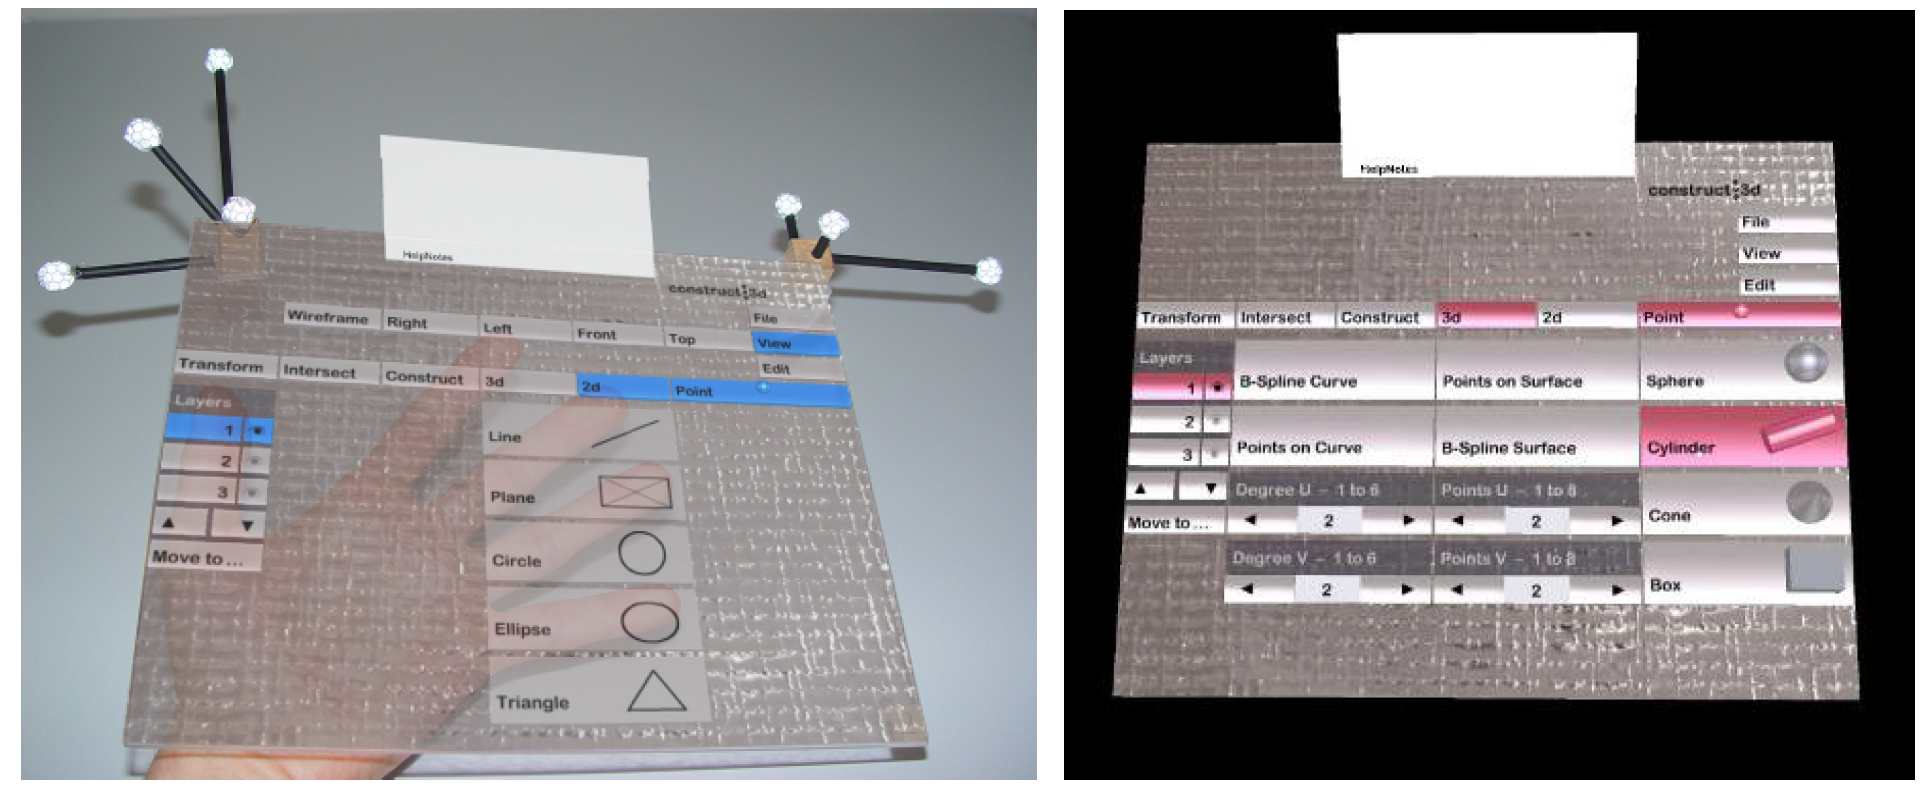
\includegraphics[scale=0.3]{Bilder/UI.PNG}
\caption{Links: Menüsystem von Construct3D, das auf dem PIP angezeigt wird. In einer Hilfebox (oben) werden weitere Details und Hilfe zu den Anwendungsfunktionen dargestellt. Rechts: 3D-Untermenü, welches der benutzenden Person angezeigt wird, die mit dem roten Farbschema arbeitet. [4, S.662]}
\label{UI}
\end{center}
\end{figure} 
Zu den Visualisierungstechniken, die in Construct3D verwendet werden, gehören die Verwendung von Transparenz, um das Verständnis der 
Benutzenden für die Konstruktion zu verbessern, die Farbcodierung, um zwischen den Beiträgen mehrerer Benutzenden zu unterscheiden, 
die Trennung in Ebenen, um die semantische Strukturierung einer Konstruktion zu unterstützen, und die automatische Vorschau neuer Objekte. 
Obwohl diese Techniken Szenenverarbeitung und grafisches Rendern trotz des einfachen Aussehens der Anwendung ziemlich teuer machen, 
ist diese zusätzliche Rechenleistung wert, da die Benutzerfreundlichkeit nach der Einführung dieser Funktionen verbessert wird. [S.3]\\
In der ersten Version von Construct3D wurde ein Schieberegler implementiert, der den Benutzenden die Möglichkeit gab, die Transparenz von 
Objekten selbst zu ändern. Dies war nicht zufriedenstellend, da viele Objekte nach einer Reihe von Transparenzveränderungen unterschiedliche 
Transparenzen hatten, was zu Verwirrung führte. Um eine konsistente Lernumgebung zu schaffen, wurden feste Transparenzwerte für alle Objekte und
 Farbschemata entworfen, sodass Objekte hinter mehr als zwei weiteren überlappenden 3D-Objekten noch zu sehen sind. Komplexe Objekte sind 
jedoch undurchsichtig gezeichnet. Es ist aber möglich, sie einzeln in den Wireframe-Modus zu schalten. [S.4]
\noindent \\
Um geometrische Inhalte zu strukturieren wurde neben der Kodierung von Benutzerinformationen im Farbschema (blau, orange, grün und rot) auch 
Wert daraufgelegt, visuelle Informationen über aktive und inaktive Ebenen zu haben, indem die Inaktiven in einem entsättigten Stil dargestellt werden. 
Dies wird in der Abb. \ref{Unterraeume} illustriert. Während aktive Objekte sich im rechten oberen Bereich jedes Bildes befinden, sind inaktiven Objekten im jeweiligen
 linken unteren Ecken zu sehen. Alle Screenshots in der ersten Zeile zeigen einen Vergleich zwischen desselektierten und inaktiven Objekten.
 In der zweiten Zeile werden die Ausgewählten mit inaktiven Ebenen verglichen. [S.4 f.]\\
\begin{figure}
\begin{center}
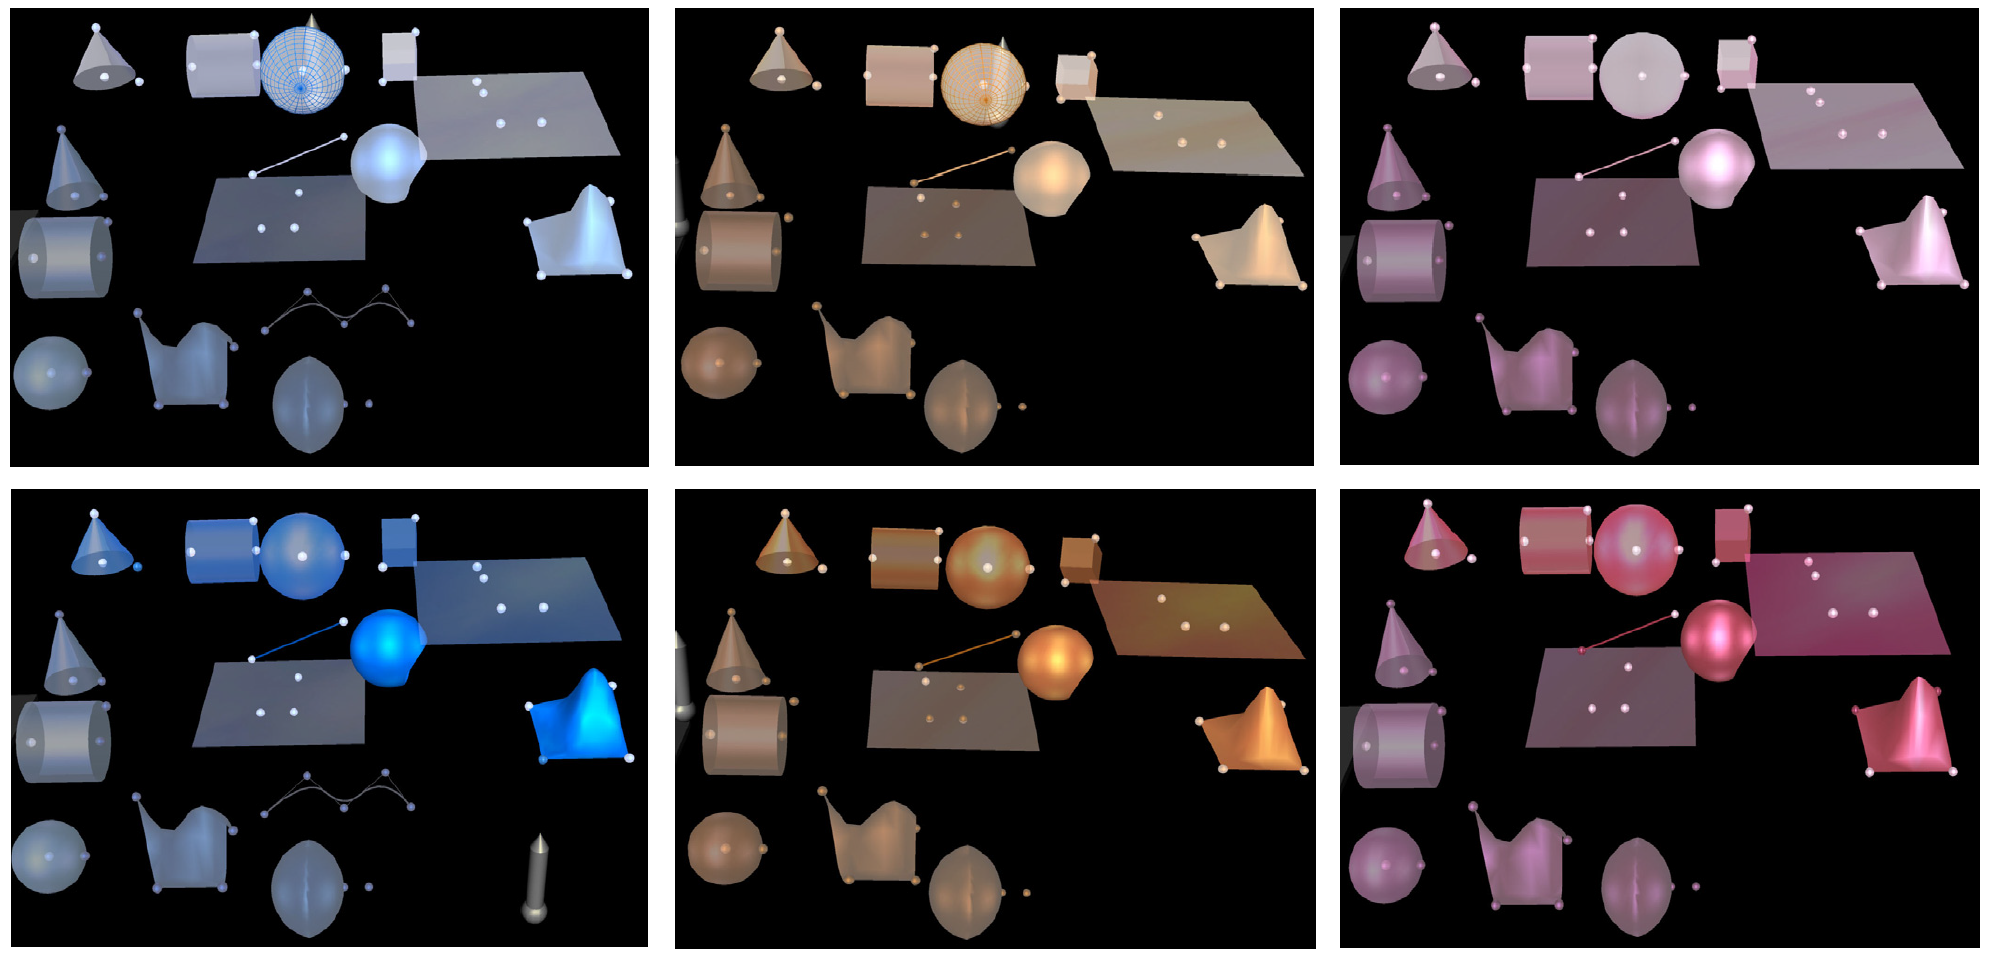
\includegraphics[scale=0.3]{Bilder/Unterraeume.PNG}
\caption{Drei Construct3D Unterräume mit Farben für ausgewählte / abgewählte / aktive und inaktive Ebenen.[S.5]}
\label{Unterraeume}
\end{center}
\end{figure}
Da die Implementierung des Farbschemas für die Farbe pro benutzende Person und die Anzeige von Ebenen sich als problematischer als ursprünglich erwartet erwies, wurde jedem Primitiv ein anderes Material zugewiesen. Insgesamt wurden mehr als 140 verschiedene Materialien für die Objekte entworfen, um ein einzigartiges Aussehen und Gefühl zu erzeugen. 6 Lichter wurden zu der Szene hinzugefügt, um einheitliche Beleuchtungsbedingungen unabhängig von der Position der Benutzenden in der virtuellen Umgebung zu erzeugen.[S.5]\\
Zusätzlich bietet Construc3D folgende Funktionen: Beim Nahekommen eines Objektes bzw. Punktes kann es hervorgehoben bzw. gezogen werden. Eine Vorschaufunktion ist ebenfalls möglich nach der visuellen Rückmeldung, dass die Konstruktion mit den Eingabeparametern funktioniert (Siehe Abb. \ref{Vorschau}).[S.5 f.]\\ 
\begin{figure}
\begin{center}
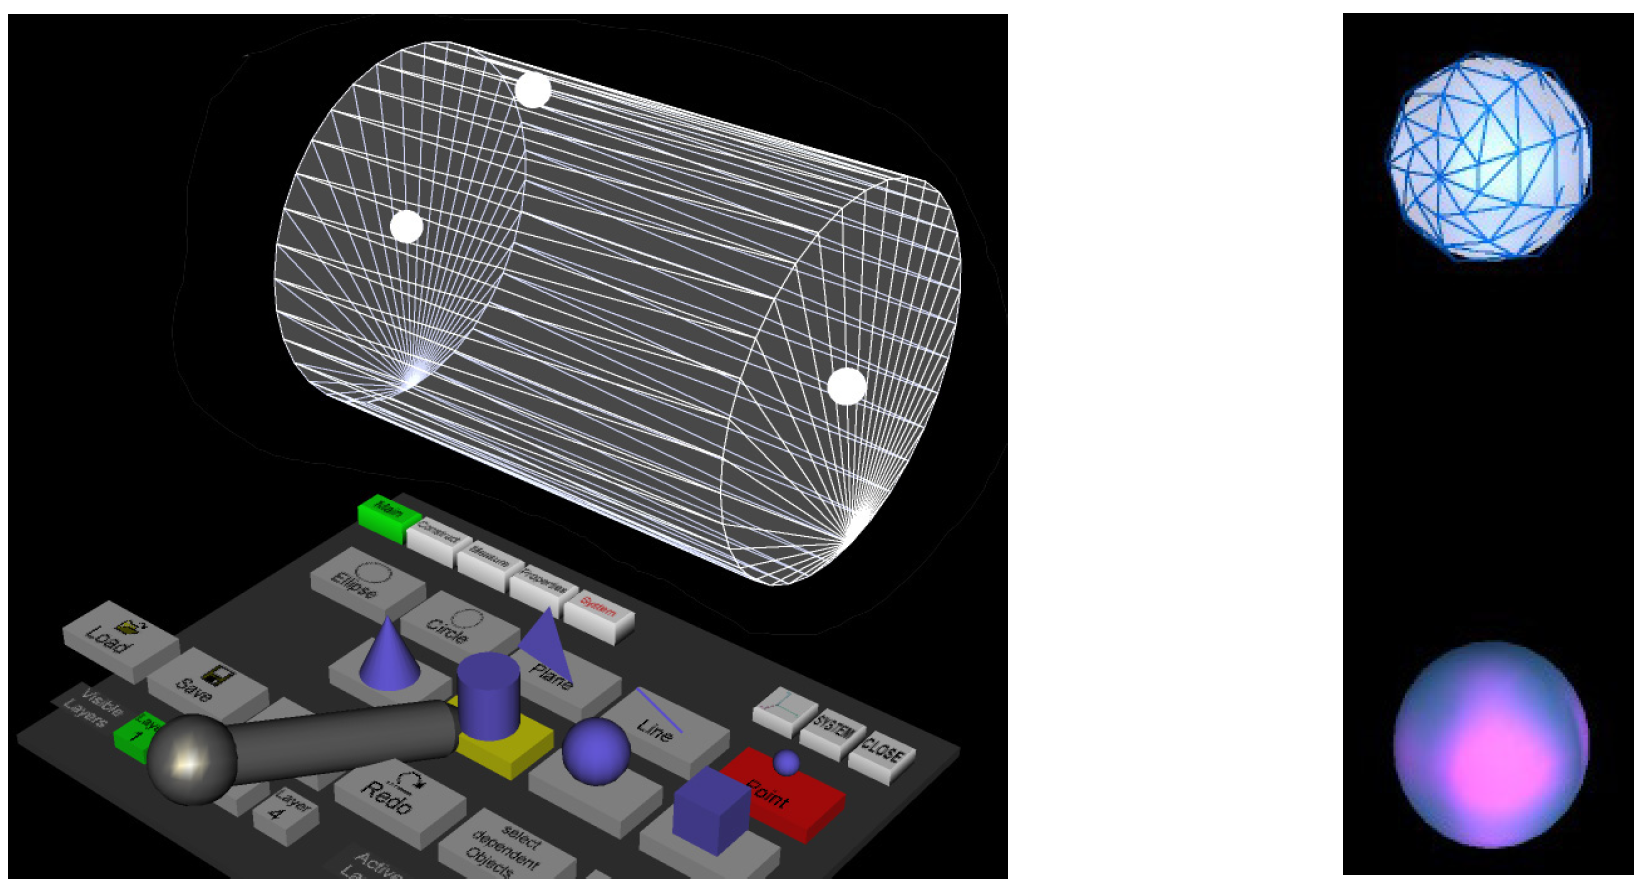
\includegraphics[scale=0.3]{Bilder/Vorschau.PNG}
\caption{Links: Vorschaue eines Zylinders. Rechts oben: Ein hervorgehobener Punkt.
Rechts unten: Ein Punkt, der gezogen werden kann. [S.6]}
\label{Vorschau}
\end{center}
\end{figure}


\subsection{Summary of Usability Evaluations of an Educational Agumented Reality Application}

Der Entwicklungsprozess von Construct3D ähnelt den Usability Engineering Methoden der virtuellen Umgebungen, die in [5] vorgeschlagen wurden [4, S.661]. Wiederholte formative Auswertungen mit mehr als 100 Lernenden führten über die Jahre hinweg zum Redesign der Anwendung und der Benutzeroberfläche [4, S.660]. Insgesamt wurden 3 Bewertungen von dieser pädagogischen Augmented-Reality-Anwendung für Geometrieunterricht durchgeführt [4, S.660]. Im Folgenden werden die Bewertungen näher betrachtet und die Ergebnisse in Bezug auf Benutzerfreundlichkeit und Simulatorkrankheit sowie Richtlinien präsentiert, wie man Augmented-Reality-Anwendungen mit kopfmontierten Displays entwirft [4, S.660].\\
Im Jahr 2000 fand die erste Bewertung mit 14 Schüler\_innen statt [4, S.663]. Diese informelle Auswertung half bei der Erstellung einer detaillierten User Task Analyse [4, S.661]. Neben der positiven Rückmeldung über die leichte Handhabbarkeit und das Design wurde Problem bei Setzen von Punkten entdeckt [4, S.663]. Als Gegenmaßnahme wurde Raster- und Gitterfunktionen eingeführt [4, S.663]. Es wurde beschlossen, dass das zurzeit statische Modellierungswerkzeug Construct3D in eine dynamische 3D-Geometrieanwendung umwandeln wird, aufgrund der Schwierigkeit bei der hochpräzisen 3D-Interaktion und des Verständnisses, dass die Lernenden davon profitieren werden [4, S.663]. \\
Im Jahr 2003 wurde eine Studie auf Basis von Interviews und dem standardisierten Usability-Fragebogen ISONORM 9241/10 durchgeführt [4, S.663]. Eine Reihe von Trainingsübungen wurde entwickelt, die zum österreichischen deskriptiven Geometrie-Curriculum der 11. und 12. Klasse passen [4, S.663].  Daran arbeiteten die Teilnehmenden (9 Schüler, 6 Schülerinnen) mit Hilfe ihrer Lehrenden [4, S.663]. Jede Person nahm an 5 Trainingseinheiten mit einer Dauer von insgesamt 6 Stunden teil [4, S.663]. Die Bewertung danach zeigte, dass die von Lernenden hoch bewerteten Kategorien (siehe Abb. \ref{Fragebogen}) auch den subjektiv gesehenen höchsten Prioritäten einer Bildungsanwendung (einfach bedienbar, schnell erlernbar; ermutigend, neues auszuprobieren; konsistent und im Gedächtnis bleibend) entsprechen [4, S.664].\\
\begin{figure}
\begin{center}
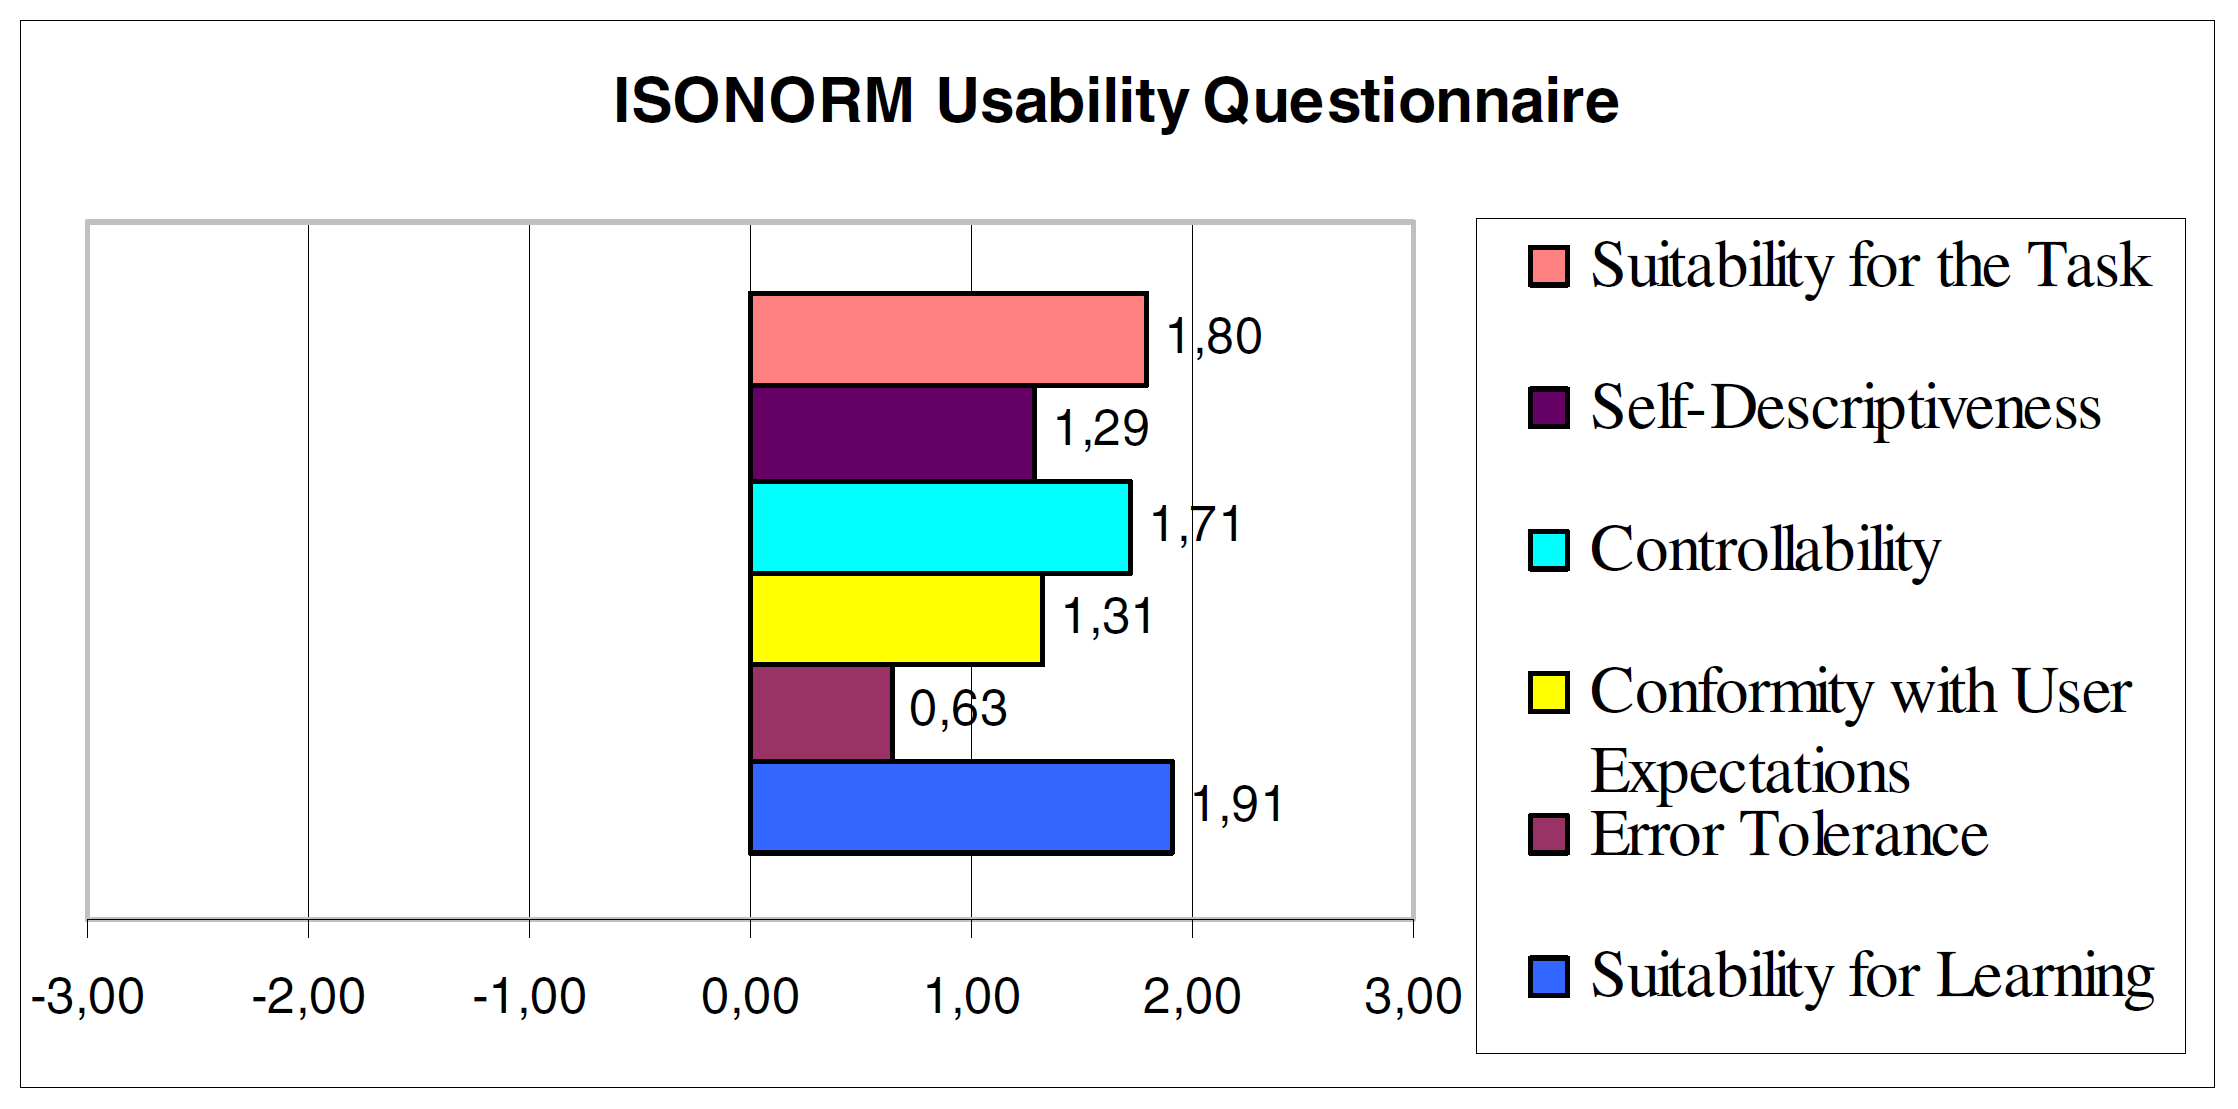
\includegraphics[scale=0.2]{Bilder/Fragebogen.PNG}
\caption{Ergebnisse des ISONORM Usability-Fragebogens in 6 Kategorien [4, S.664]}
\label{Fragebogen}
\end{center}
\end{figure}
Um die Selbstbeschreibbarkeit von Construct3D zu verbessern, wurden bessere Beschriftungen hinzugefügt, sowie eine Hilfe-Box auf dem Panel, um alle Menüelemente zu erklären [4, S.664]. Neben der neuen Strukturierung des Menüsystems wurde das visuelle Design von geometrischen Objekten auch verbessert [4, S.664]. Eingeführt wurden Transparenz-Verwendung, konsistente Farbcodierung, Ebene-Trennung und automatische Vorschau neuer Objekte [4, S.664]. Nähere Informationen zu den Verbesserungen siehe \textit{Designing Immersive Virtual Reality for Geometry Education.}\\
Die dritte Auswertung war im Jahr 2005 [4, S.665]. Verglichen wurde das Lösen von geometrischen Problemen mit Construct3D mit einer pädagogischen Desktop-Anwendung namens CAD3D [4, S.665]. Teilnehmenden waren österreichische Oberstufenschüler\_innen im Alter zwischen 16 und 19 Jahren (M = 17,49, SD = .79; 44 (48,4\%) männlich und 47 (51,6\%) weiblich) [4, S.665]. Sie nahmen an 6 Trainingseinheiten teil, die 45 Minuten dauerten [4, S.665]. In beiden Gruppen betreute ein Tutor oder eine Tutorin zwei Lernenden beim Arbeiten an den Geometrieaufgaben [4, S.665]. Zur Beurteilung der Benutzerfreundlichkeit wurden Fragenbogen entwickelt, die von 8 etablierten Usability-Fragebögen angepasst waren (7 Skalen (siehe Abb. \ref{Bewertung}); insgesamt 28 Fragen) [4, S.665].\\
\begin{figure}
\begin{center}
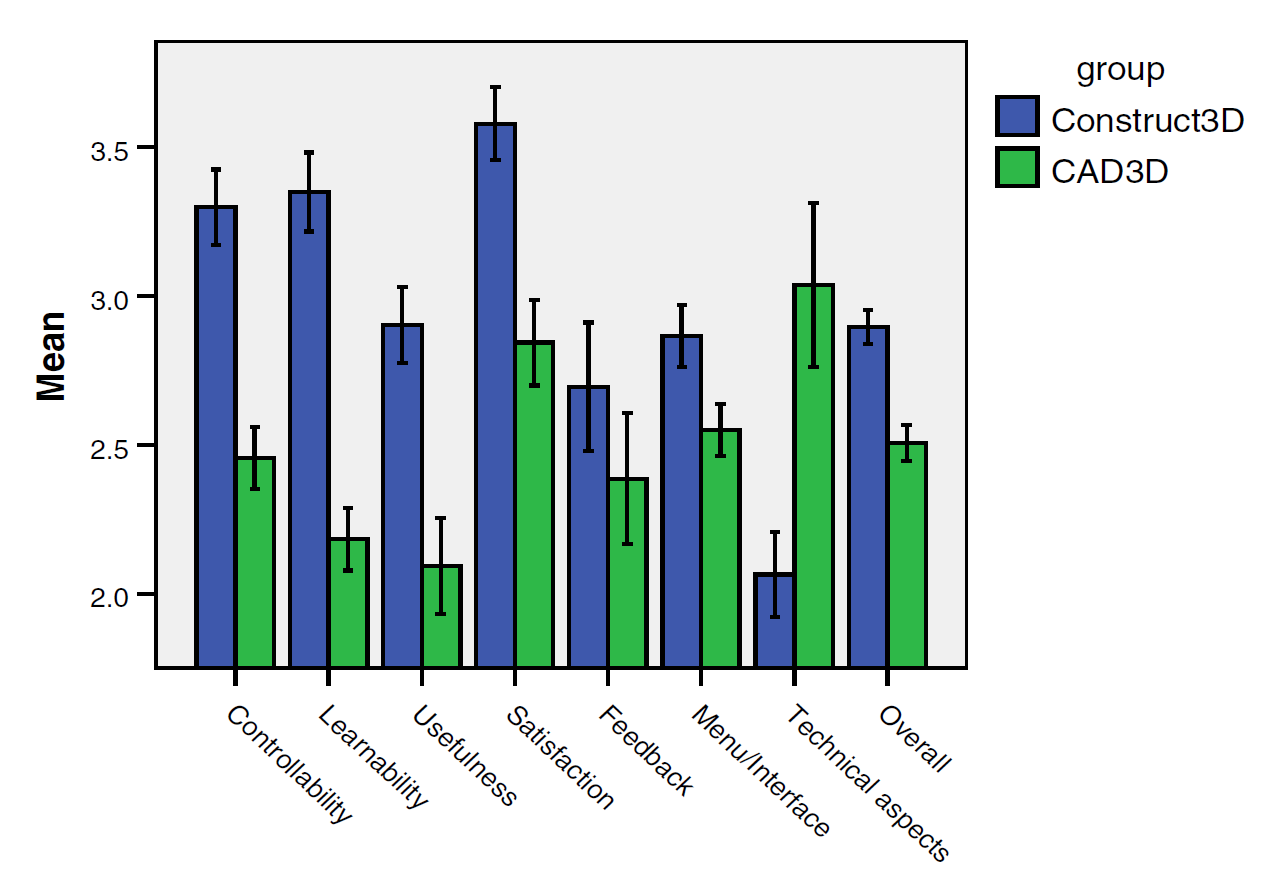
\includegraphics[scale=0.4]{Bilder/Bewertung.PNG}
\caption{Usability-Bewertungen von Lernenden bezüglich der Verwendung von Construct3D und CAD3D (4-Punkt-Likert-Skala; 1-min, 4-max = am besten; Fehlerbalken $\pm$ 1,96 * Standardfehler) [4, S.665]}
\label{Bewertung}
\end{center}
\end{figure}
Die Analyse der Fragenbogen ergab, dass Construct3D ein hochgradig benutzerfreundliches System ist, das - aus Usability-Sicht - mehrere Vorteile gegenüber der traditionellen Desktop-basierten Anwendung aufweist [4, S.666]. Die niedrigen Bewertungen für technische Aspekte deuten jedoch darauf hin, dass es noch Probleme bezüglich der technischen Robustheit gibt, die angegangen werden müssen [4, S.666]. Seltene Systemabstürze und kleinere technische Probleme können die Motivation der Teilnehmer und die Benutzerfreundlichkeit des Systems beeinträchtigen [4, S.666]. Construct3D sollte hauptsächlich für Lehrinhalte verwendet werden, die eine dynamische 3D-Geometrie verwenden oder die Visualisierung abstrakter Probleme erfordern [4, S.666]. In Bezug auf die bevorzugte Trainingseinrichtung der Lernenden zwischen Construct3D und CAD3D gab es keine signifikanten Unterschiede [4, S.666]. Die Mehrheit der Lernenden möchte Construct3D in der Schule einsetzen (ja = 64,44\%, eher ja = 26,67\%); 8,89\% möchten das System lieber nicht in der Schule einsetzen [4, S.666].  Die Kommentare zu den potenziellen Problemen beim Einsatz von Construct3D in Schulen betrafen vor allem fehlende Finanzierung und die Robustheit der Hardware und Software [4, S.666].\\

\textbf{Simulator Sickness}\\
In der Evaluationsstudie im Jahr 2003 wurde diese negative Nebenwirkung von einigen Lernenden berichtet [4, S.667]. 20 Minuten nach dem Beginn des Arbeitens in der virtuellen Umgebung tauchen Kopfschmerzen und Augenbelastungen bei einer Schülerin auf, trotzdem wollte sie damit weiterarbeiten [4, S.667]. Im Nachhinein stellt es sich heraus, dass die einstündigen Auswertungen für die kontinuierliche Arbeit mit einem HMD zu lang waren [4, S.667]. Da negative Nebenwirkungen ein allgemeines potenzielles Problem bei der Arbeit mit HMDs darstellen und die subjektive Erfahrung der Benutzenden erheblich beeinflussen, sind sie für alle VR/AR-Anwendungen relevant, die diese Displays verwenden [4, S.667]. Mögliche Gründe für diese Nebenwirkung wären Akkomodationsprobleme, niedrige Bildfrequenz, Verzögerung oder schlechtsitzende Helme [4, S.667].\\
Folglich wurde in der dritten Studie im Jahr 2005 die Trainingsdauer pro Einheit auf maximal 45 Minuten reduziert, Hartplastikhelm durch leichten Fahrradhelm ersetzt und selbstbestimmte Ausruhzeit eingeführt [4, S.667 f.]. Trotzdem spürten 75,56\% der 47 Teilnehmenden eine moderate Müdigkeit oder Erschöpfung und 61,36\% berichteten von einer leichten Augenbelastung [4, S.668]. Einige hatten Kopfschmerzen (37,78\%) und Schwindelgefühl (35,56\%) (siehe Abb. \ref{Sickness}) [4, S.668]. Im Allgemeinen berichteten die meisten Teilnehmenden jedoch nicht, dass sie schwerwiegende Probleme hatten [4, S.668]. Die meisten dieser Symptome könnten mit der Verwendung einer HMD zusammenhängen [4, S.668]. In Übereinstimmung mit den Beobachtungen und anderen Studien wurde empfohlen, die HMD-Nutzungszeit auf 20-30 Minuten pro Einheit zu beschränken [4, S.668]. Basierend auf der Erfahrung trägt die Bildqualität von HMDs, insbesondere die Verzögerung und Qualität der Tracking-Daten, am meisten zu den berichteten Effekten bei [4, S.668].\\
\begin{figure}
\begin{center}
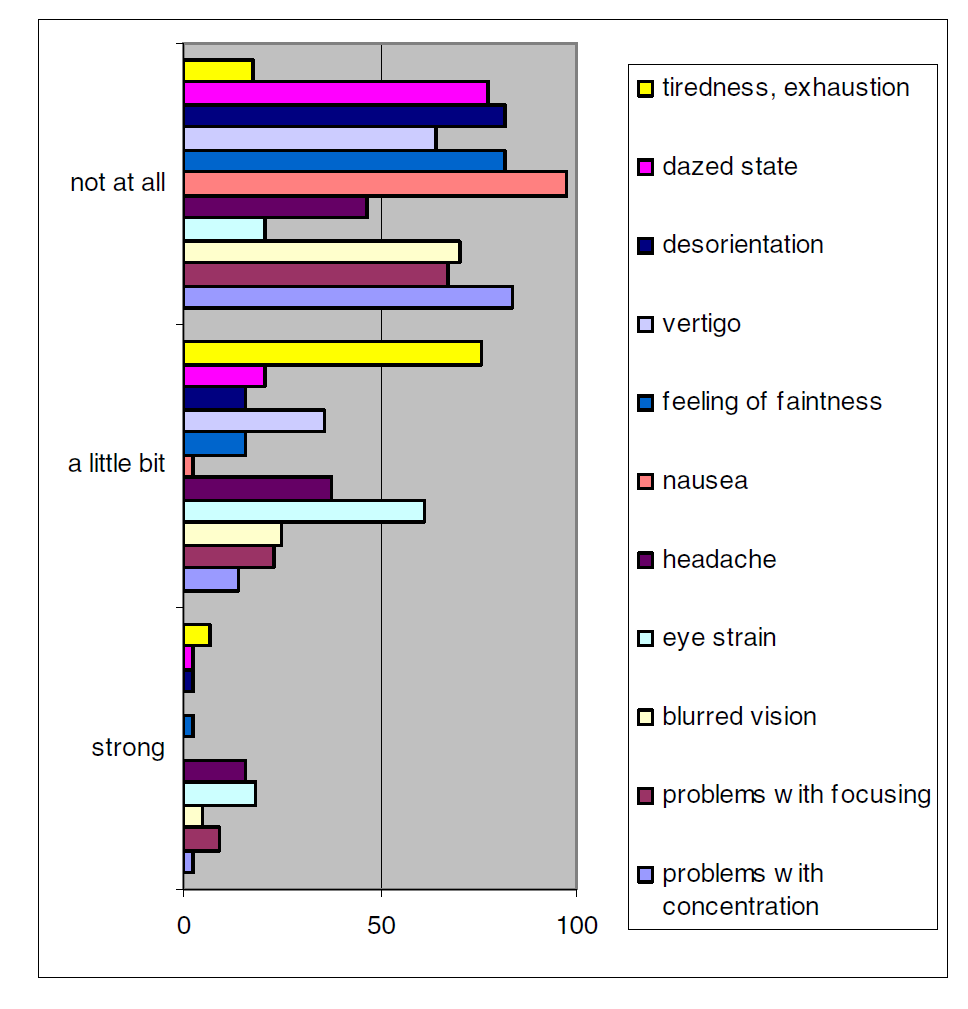
\includegraphics[scale=0.5]{Bilder/Sickness.PNG}
\caption{Prozentsatz der Benutzenden, die ein bestimmtes Symptom melden, wird angezeigt (0\% = von keiner benutzenden Person gemeldet; 100\% = von allen Benutzenden gemeldet) [4, S.668].}
\label{Sickness}
\end{center}
\end{figure}

\section{Zusammenfassung}
\label{sec:typo}
In dieser Zusammenfassung .... 

\section{Literaturverzeichnis}
\label{sec:bib}

\subsection{Literatursuche}
\label{subsec:search}


\subsection{BibTeX}
\label{subsec:bibtex}
[1] https://www.vrnerds.de/die-geschichte-der-virtuellen-realitaet/
\cite{2 http://virtualrealityforeducation.com/wp-content/uploads/2018/06/HuAu_Lee_2017_VRinEd.pdf}
TY  - BOOK
AU  - Kaufmann, Hannes
PY  - 2003/03/20
SP  - 
T1  - Collaborative Augmented Reality in Education
ER  - 
\printbibliography

[5] Hix, D., Gabbard, J.L.: Usability Engineering of Virtual Environments. In: Stanney, K.M.
(ed.) Handbook of Virtual Environments - Design, Implementation, and Applications, pp.
681–699. Lawrence Erlbaum Associates, Mahwah, New Jersey (2002)


\end{document}